\documentclass[final]{beamer}

\usepackage[size=a0,orientation=landscape,scale=1.15]{beamerposter}
\usepackage[T1]{fontenc}
\usepackage[utf8]{inputenc}
\usepackage{lmodern}
\usepackage{listings}
\usefonttheme{serif}
\usepackage{amsmath,amssymb}
\usepackage{array}
\usepackage{graphicx}
\usepackage{tikz}
\usepackage[most]{tcolorbox}
\usetikzlibrary{arrows.meta,positioning}

\usetheme{default}
\setbeamertemplate{navigation symbols}{}

\definecolor{posterblue}{RGB}{25,61,102}
\definecolor{posterlight}{RGB}{247,249,252}
\definecolor{posterline}{RGB}{224,229,236}
\definecolor{posterink}{RGB}{35,45,58}

\setbeamercolor{background canvas}{bg=white}
\setbeamercolor{normal text}{fg=posterink}
\setbeamertemplate{itemize item}{\color{posterink}$\bullet$}
\setbeamerfont{title}{size=\fontsize{85}{98}\selectfont,series=\bfseries}
\setbeamerfont{subtitle}{size=\fontsize{36}{44}\selectfont,series=\bfseries}
\setbeamerfont{author}{size=\fontsize{24}{31}\selectfont}
\setbeamerfont{block title}{size=\fontsize{36}{44}\selectfont,series=\bfseries}
\setbeamerfont{block body}{size=\fontsize{24}{31}\selectfont}

\newcommand{\posterbodyfont}{\fontsize{24}{31}\selectfont}
\newcommand{\postercompactfont}{\fontsize{22}{28}\selectfont}
\newcommand{\posterdensefont}{\fontsize{20}{25}\selectfont}
\newcommand{\postercaptionfont}{\fontsize{18}{23}\selectfont}

\newtcolorbox{posterbox}[2][]{%
  enhanced,
  colback=posterlight,
  colframe=posterline,
  coltitle=white,
  colbacktitle=posterblue,
  fonttitle=\usebeamerfont{block title},
  fontupper=\usebeamerfont{block body},
  title={#2},
  titlerule=0pt,
  toptitle=0.18cm,
  bottomtitle=0.18cm,
  left=0.55cm,
  right=0.55cm,
  top=0.48cm,
  bottom=0.35cm,
  arc=3mm,
  boxrule=0.8pt,
  valign=center,
  #1
}

\newtcolorbox{mathbox}[1][]{%
  enhanced,
  colback=white,
  colframe=posterline,
  boxrule=0.6pt,
  arc=2mm,
  left=0.28cm,
  right=0.28cm,
  top=0.18cm,
  bottom=0.18cm,
  #1
}

\tcbset{
  compactboxtitle/.style={
    fonttitle={\usebeamerfont{block title}},
    toptitle=0.11cm,
    bottomtitle=0.05cm
  }
}

\newcommand{\systemdiagram}{%
  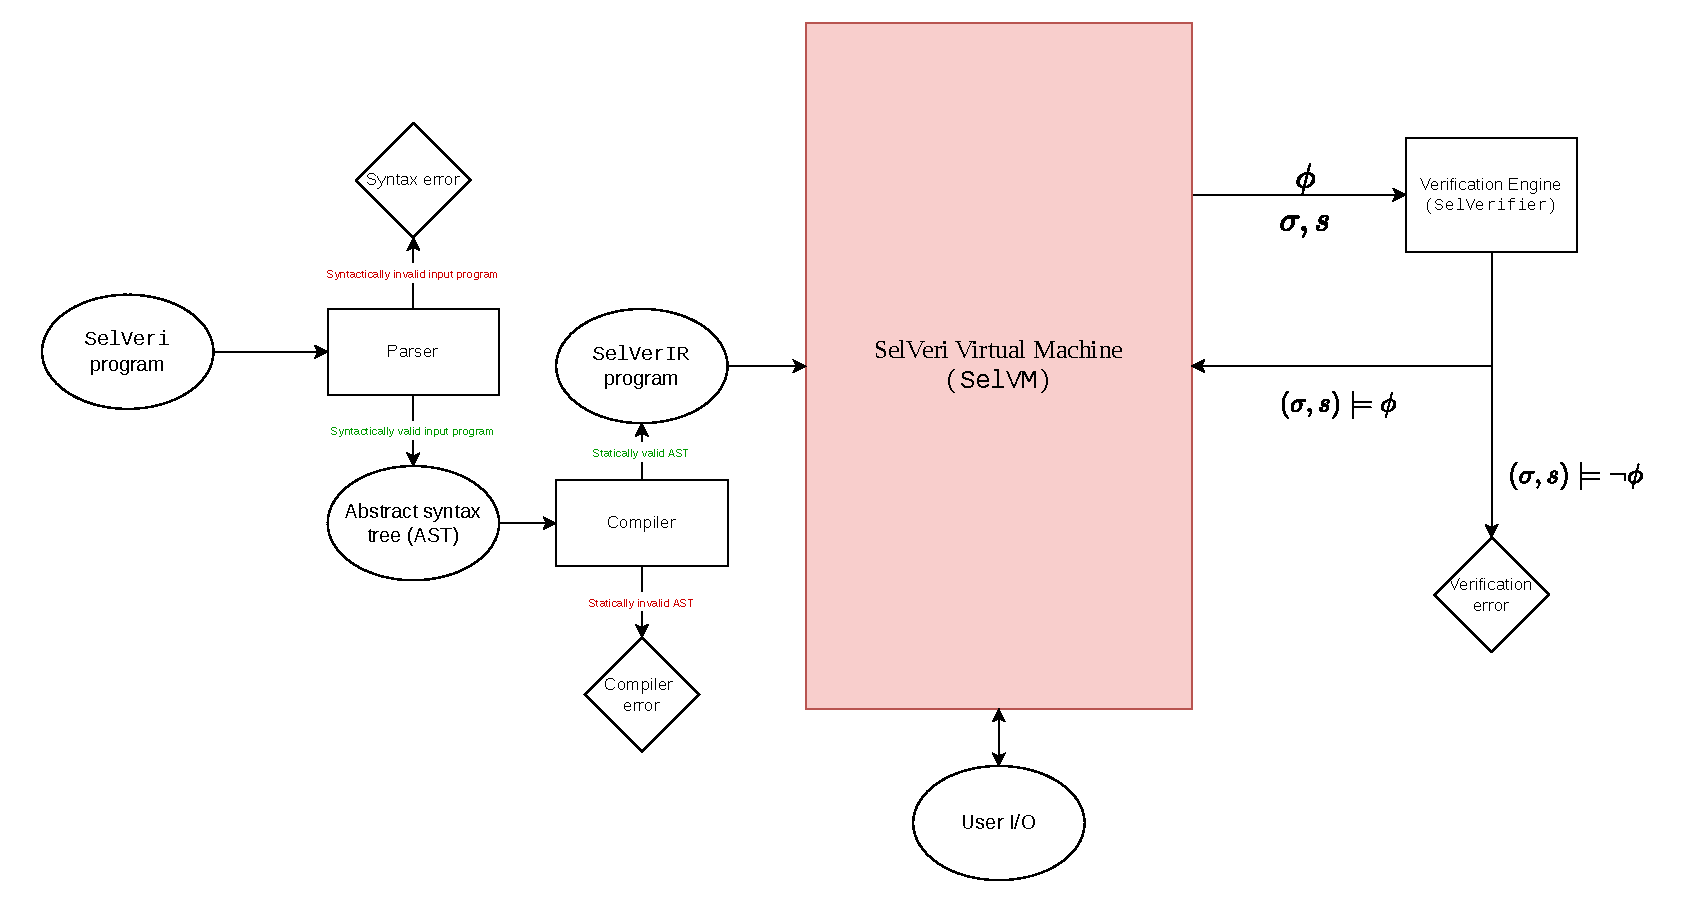
\includegraphics[width=\linewidth,height=11.5cm,keepaspectratio]{visuals/SelVeri-system_diagram.pdf}%
}

\title{SelVeri}
\subtitle{Self-Verifying Programming Language}
\author{Yağız Kaan Aydoğdu \textperiodcentered{} Yusuf Demir \textbar{} Advisor: Doğan Ulus}

\begin{document}
\begin{frame}[t,fragile]

\begin{tcolorbox}[
  enhanced,
  width=\textwidth,
  height=7.4cm,
  colback=posterblue,
  colframe=posterblue,
  boxrule=0pt,
  arc=0pt,
  left=0pt,
  right=0pt,
  top=0.35cm,
  bottom=0pt,
]
\begin{minipage}[c]{0.15\textwidth}
  \centering
  
\includegraphics[height=6.2cm]{visuals/boun_logo.png}
\end{minipage}%
\begin{minipage}[c]{0.68\textwidth}
  \centering
  {\usebeamerfont{title}\color{white}\inserttitle\par}
  \vspace{0.18cm}
  {\usebeamerfont{subtitle}\color{white}\insertsubtitle\par}
  \vspace{0.25cm}
  {\usebeamerfont{author}\color{white}\insertauthor\par}
 \end{minipage}%
\begin{minipage}[c]{0.15\textwidth}
  \hfill
\end{minipage}
\end{tcolorbox}

\vspace{0.2cm}

\begin{columns}[t,totalwidth=\textwidth]

\begin{column}{0.245\textwidth}

\begin{posterbox}[height=23cm,compactboxtitle]{Project Overview}
{\postercompactfont
\begin{itemize}
  \setlength{\itemsep}{0.03cm}
  \item SelVeri is an educational imperative language that \textbf{connects sequential programming with formal methods}.

  \item Programs may contain \textbf{first-order logic} or \textbf{linear temporal logic} specifications that are checked dynamically as execution reaches verification points.

  \item The implementation parses high-level programs, compiles into the intermediate representation, which is executed on a stack-based abstract machine.

  \item The verification engine translates runtime configurations to mathematical constraints and uses them to verify logical specifications.
\end{itemize}
}

\vspace{-0.05cm}
\begin{center}
  \systemdiagram
\end{center}
\end{posterbox}

\vspace{0.25cm}

\begin{posterbox}[height=16.8cm,compactboxtitle]{Syntax}
{\postercaptionfont
\begin{mathbox}[left=0.25cm,right=0.25cm,top=0.28cm,bottom=0.28cm]
\[
\renewcommand{\arraystretch}{1.18}
\begin{array}{rcl}
P &::=& F^*\,S^* \\[3pt]
F &::=& \mathtt{function}\ f(\overline{x:T}) \to T\ \mathtt{::}\ S^*\ \mathtt{end} \\[3pt]
T &::=& \tau \mid \mathtt{List}[\tau,d,\overline{A}],
\qquad \tau ::= \mathtt{Int}\mid\mathtt{Real} \\[3pt]
S &::=& x:T \mid x:=A \mid x[A]:=A \mid \mathtt{pass}
\mid \mathtt{call}\ f(\overline{A}) \\[1pt]
&\mid& \mathtt{write}(A) \mid \mathtt{writeline}(A)
\mid \mathtt{return}\ A \mid \{\mathit{Spec}\} \\[1pt]
&\mid& \mathtt{if}\ B\ \mathtt{then}\ S^*
[\mathtt{else}\ S^*]\ \mathtt{fi} \\[1pt]
&\mid& \mathtt{while}\ B\ \mathtt{do}\ S^*\ \mathtt{od} \\[3pt]
A &::=& n \mid r \mid x \mid [\overline{A}]
\mid A\oplus A \mid -A
\mid x[A] \mid \mathtt{len}(x) \mid \mathtt{read}() \\[1pt]
&\mid& \mathtt{obtain}(\&x,\mathit{Spec}) \\[3pt]
B &::=& \mathtt{true} \mid \mathtt{false}
\mid A\bowtie A \mid \mathtt{not}\ B
\mid B\circ B \mid \{\mathit{Spec}\}
\end{array}
\]
\end{mathbox}

\vspace{0.12cm}
\begin{center}
{\postercaptionfont Simplified syntax of SelVeri in Backus-Naur Form.}
\end{center}

\vspace{-0.05cm}
\begin{itemize}
  \item Actual syntax is more sophisticated to impose implementation details, such as operator precedence.
\end{itemize}
}
\end{posterbox}

\vspace{0.25cm}

\begin{posterbox}[height=26.6cm,compactboxtitle]{Semantics}
{\posterbodyfont
\begin{mathbox}[left=0.25cm,right=0.25cm,top=0.2cm,bottom=0.2cm]
\textbf{Configuration}
\[
\gamma = \langle S,\sigma,s,\iota,\Omega\rangle
\]
\vspace{-0.25cm}
\begin{center}
\renewcommand{\arraystretch}{1.08}
\begin{tabular}{>{$}r<{$}p{0.74\linewidth}}
\sigma & program state, mapping variables to values \\
s      & scope, mapping variables to declared types \\
\iota  & input stream consumed by \(\mathtt{read}()\) \\
\Omega & output and verification trace
\end{tabular}
\end{center}
\end{mathbox}

\vspace{0.18cm}
\begin{mathbox}[left=0.25cm,right=0.25cm,top=0.2cm,bottom=0.2cm]
\textbf{Small-Step Rules}
\[
\renewcommand{\arraystretch}{1.0}
\begin{array}{rcl}
\langle x:T,\sigma,s\rangle
&\to&
\langle \sigma[x\mapsto \mathbf{0}_T],\,s[x\mapsto T]\rangle \\
\langle x:=A,\sigma,s\rangle
&\to&
\langle \sigma[x\mapsto \mathcal{A}(A,\sigma,s,\iota)],\,s\rangle \\
\langle \mathtt{if}\ b\ \mathtt{then}\ S_1\ \mathtt{else}\ S_2,\sigma,s\rangle
&\to&
\begin{cases}
\langle S_1,\sigma,s\rangle & \mathcal{B}(b,\sigma,s)=1\\
\langle S_2,\sigma,s\rangle & \mathcal{B}(b,\sigma,s)=0
\end{cases} \\
\langle \mathtt{while}\ b\ \mathtt{do}\ S,\sigma,s\rangle
&\to&
\begin{cases}
\langle S;\mathtt{while}\ b\ \mathtt{do}\ S,\sigma,s\rangle
& \mathcal{B}(b,\sigma,s)=1\\
\langle \sigma,s\rangle
& \mathcal{B}(b,\sigma,s)=0
\end{cases}
\end{array}
\]
\end{mathbox}

\vspace{0.15cm}
\begin{itemize}
  \item $\mathcal{A}$ evaluates arithmetic expressions; $\mathcal{B}$ evaluates boolean guards as $1$ or $0$.
  \item Declarations extend scope; assignments update state; undefined configurations enter erroneous program state, $\hat{\sigma}$.
\end{itemize}
}
\end{posterbox}
\end{column}

\begin{column}{0.245\textwidth}

\begin{posterbox}[height=21.7cm,compactboxtitle]{Compilation to SelVerIR}
{\posterdensefont
\[
\begin{aligned}
\mathcal{C}&:\mathbf{Code}_{\text{SelVeri}}\to\mathbf{Code}_{\text{IR}},&
\mathcal{CA}&:\mathbf{AExp}\to\mathbf{Code}_{\text{IR}},\\
\mathcal{CB}&:\mathbf{BExp}\to\mathbf{Code}_{\text{IR}}
\end{aligned}
\]

\vspace{0.05cm}
\begin{center}
\renewcommand{\arraystretch}{1.04}
\begin{tabular}{p{0.31\linewidth}p{0.58\linewidth}}
\textbf{SelVeri fragment} & \textbf{SelVerIR emitted} \\
\hline
$a$ & $\mathcal{CA}(a)$ leaves the value of $a$ on stack $e$ \\
$b$ & $\mathcal{CB}(b)$ leaves $1$ or $0$ on stack $e$ \\
$x:T$ & $\mathtt{DECL}\ T\ x$ \\
$x:=a$ & $\mathcal{CA}(a):\mathtt{STORE}\ x$ \\
$S_1;S_2$ & $\mathcal{C}(S_1):\mathcal{C}(S_2)$ \\
$\mathtt{if}\ b\ \mathtt{then}\ S_1\ \mathtt{else}\ S_2$ &
$\mathcal{CB}(b):\mathtt{JZ}\ L_e:\mathcal{C}(S_1):\mathtt{GOTO}\ L_o:L_e:\mathcal{C}(S_2):L_o$ \\
$\mathtt{while}\ b\ \mathtt{do}\ S$ &
$L_h:\mathcal{CB}(b):\mathtt{JZ}\ L_o:\mathcal{C}(S):\mathtt{GOTO}\ L_h:L_o$
\end{tabular}
\end{center}

\vspace{0.05cm}
\begin{itemize}
  \item The compiler emits labeled stack-machine commands; labels become concrete program counters after jump patching.
\end{itemize}

\vspace{-0.1cm}
\begin{mathbox}[left=0.25cm,right=0.25cm,top=0.18cm,bottom=0.18cm]
\begin{center}
\renewcommand{\arraystretch}{1.03}
\begin{tabular}{c@{\hspace{0.35cm}}c@{\hspace{0.35cm}}c}
\textbf{SelVeri program} & $\Longrightarrow$ & \textbf{SelVerIR program} \\
\begin{tabular}{l}
\texttt{x : Int;} \\
\texttt{x := 3 + 4;} \\
\texttt{write(x);}
\end{tabular}
&
&
\begin{tabular}{l}
\texttt{DECL INT x} \\
\texttt{PUSH 3 : PUSH 4 : ADD : STORE x} \\
\texttt{LOAD x : WRITE}
\end{tabular}
\end{tabular}
\end{center}
\end{mathbox}
}
\end{posterbox}

\vspace{0.25cm}

\begin{posterbox}[height=19.5cm,compactboxtitle]{\shortstack[l]{Logic Programming Extension: SelVeri LP}}
{\posterbodyfont
\begin{itemize}
  \item SelVeri LP \textbf{closes the gap between imperative programming and logic/declarative programming}.

  \item Specifications can act as boolean guards in ordinary control flow:
\end{itemize}
\vspace{-0.2cm}
\begin{mathbox}[left=0.35cm,right=0.35cm,top=0.18cm,bottom=0.18cm]
\begin{center}
\begin{tabular}{l}
\texttt{if \{ Historically y >= x + z => b != 0 \} then} \\
\texttt{\ \ b := 1;} \\
\texttt{else} \\
\texttt{\ \ b := 0;} \\
\texttt{fi}
\end{tabular}
\end{center}
\end{mathbox}
\vspace{-0.15cm}
\begin{itemize}
  \item \texttt{obtain} asks Z3 to extract a witness satisfying a logical specification, then stores it in program state:
\end{itemize}
\vspace{-0.2cm}
\begin{mathbox}[left=0.35cm,right=0.35cm,top=0.18cm,bottom=0.18cm]
\begin{center}
\begin{tabular}{l}
\texttt{x := obtain(\&x,} $\exists$ \texttt{y} $\in$ \texttt{Int.} \&y = n*n*n\texttt{)} \\
\end{tabular}
\end{center}
\end{mathbox}
}
\end{posterbox}

\vspace{0.25cm}

\begin{posterbox}[height=25.21cm,compactboxtitle]{Proven Properties of SelVeri}
{\posterbodyfont
\begin{mathbox}[left=0.28cm,right=0.28cm,top=0.24cm,bottom=0.24cm]
\textbf{Correctness of Compilation}
\vspace{0.1cm}
\begin{center}
\renewcommand{\arraystretch}{1.12}
\begin{tabular}{p{0.32\linewidth}p{0.56\linewidth}}
\textbf{Expressions} & structural induction on the syntactic structure of expressions \\
\textbf{Terminating} & strong induction on execution length \\
\textbf{Divergent} & transfinite induction  on exectuion length while utilizing the $\omega$-bound of computation
\end{tabular}
\end{center}
\end{mathbox}

\vspace{0.25cm}
\begin{mathbox}[left=0.28cm,right=0.28cm,top=0.24cm,bottom=0.24cm]
\begin{center}
\renewcommand{\arraystretch}{1.14}
\begin{tabular}{p{0.32\linewidth}p{0.56\linewidth}}
\textbf{Turing complete} & SelVeri can represent every general $(\mu)$-recursive function \\
\textbf{Sound verifier} & accepted encodings satisfy the source specification \\
\textbf{Deterministic} & each valid configuration has at most one next state
\end{tabular}
\end{center}
\end{mathbox}

\vspace{0.12cm}
\begin{center}
{\postercaptionfont Verified compilation transfers Turing-completeness and determinism to SelVerIR.}
\end{center}
}
\end{posterbox}
\end{column}

\begin{column}{0.245\textwidth}
\begin{posterbox}[height=16cm,compactboxtitle]{\shortstack[l]{FOL Verification with Z3 Theorem Prover}}
{\posterbodyfont
\begin{itemize}
  \item \texttt{Z3Mapper} maps the runtime configuration and FOL specification into equivalent Z3 inputs.
  \item \texttt{free\_var\_map} resolves program variables; \texttt{bound\_var\_map} resolves quantified variables.
\end{itemize}

\vspace{0.15cm}
\begin{mathbox}[left=0.25cm,right=0.25cm,top=0.18cm,bottom=0.18cm]
\[
\mathtt{VERI}\ \phi\ \text{ succeeds iff }\ 
\mathcal{M}_{\mathtt{Z3}}(\sigma,s)\models\mathcal{ZF}(\phi)
\]
\end{mathbox}

\vspace{1.45cm}
\begin{center}
\begin{tikzpicture}[
  node distance=0.72cm and 0.62cm,
  every node/.style={font=\postercaptionfont},
  flow/.style={draw,rounded corners=1.5mm,fill=white,minimum height=1.28cm,minimum width=3.05cm,align=center,line width=0.85pt},
  midflow/.style={flow,minimum width=5.95cm},
  solverflow/.style={flow,minimum width=7.55cm},
  edge/.style={->,line width=1.15pt,shorten >=1.2pt,shorten <=1.2pt},
  >={Latex[length=3.45mm,width=2.6mm]},
  scale=1.0,
  transform shape
]
\node[flow] (cfg) {$\sigma,s$\\ state + scope};
\node[flow,below=0.42cm of cfg] (spec) {$\phi$\\ FOL spec};
\node[flow,right=0.62cm of cfg,yshift=-0.78cm] (mapper) {\texttt{Z3Mapper}\\ maps to Z3};
\node[midflow,right=0.62cm of mapper,yshift=0.78cm] (mz3) {$\mathcal{M}_{\mathtt{Z3}}(\sigma,s)$, solver state};
\node[midflow,right=0.62cm of mapper,yshift=-0.78cm] (zf) {$\mathcal{ZF}(\phi)$, Z3 formula};
\node[solverflow,right=0.62cm of mz3,yshift=-0.78cm] (solver) {$\mathcal{M}_{\mathtt{Z3}}\overset{?}{\vdash}\mathcal{ZF}(\phi)$\\ entailment check};
\node[flow,right=0.62cm of solver] (res) {$\sigma$ / $\hat{\sigma}$\\ pass / fail};

\draw[edge] (cfg) -- (mapper);
\draw[edge] (spec) -- (mapper);
\draw[edge] (mapper) -- (mz3);
\draw[edge] (mapper) -- (zf);
\draw[edge] (mz3) -- (solver);
\draw[edge] (zf) -- (solver);
\draw[edge] (solver) -- (res);
\end{tikzpicture}
\end{center}
}
\end{posterbox}

\vspace{0.25cm}

\begin{posterbox}[height=18.2cm,compactboxtitle]{Past-LTL Verification}
{\posterdensefont
\begin{itemize}
  \setlength{\itemsep}{0.03cm}
  \item Past-LTL specifications are evaluated over the finite history of runtime snapshots.

  \item SelVerifier stores memoized truth values for temporal subformulae, forming a \textbf{sequential network over time}.
\end{itemize}

\vspace{0.1cm}
\begin{center}
\begin{tabular}{@{}m{0.27\linewidth}@{\hspace{0.35cm}}m{0.06\linewidth}@{\hspace{0.35cm}}m{0.58\linewidth}@{}}
\centering
{\posterdensefont
\texttt{Once(Historically p}\\
\texttt{\&\& (q Since r))}
}
&
\centering{\posterdensefont $\Rightarrow$}
&
\centering
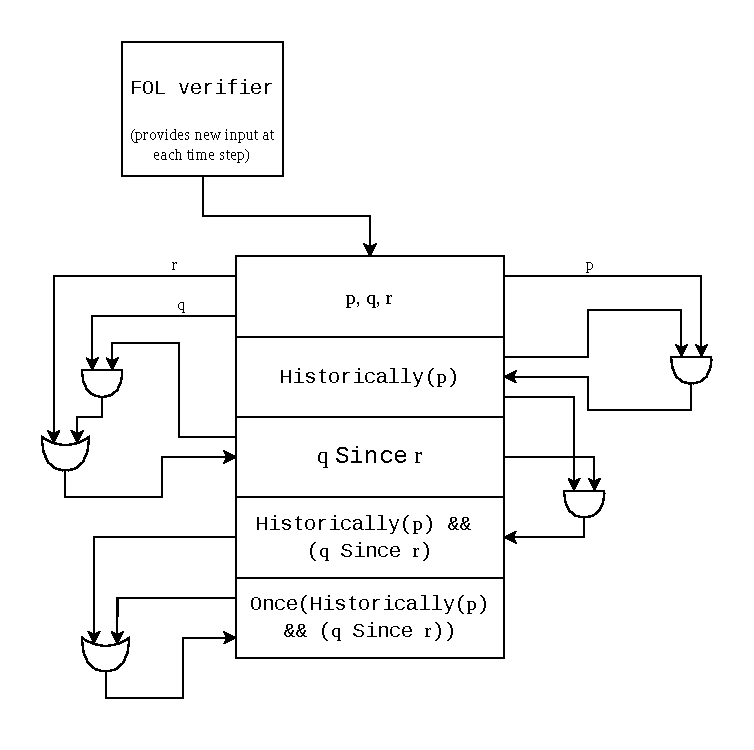
\includegraphics[width=\linewidth,height=11.8cm,keepaspectratio,trim=0.15cm 0.15cm 0.15cm 0.15cm,clip]{visuals/pltl_sequential_network.pdf}
\end{tabular}
\end{center}
}
\end{posterbox}

\vspace{0.25cm}

\begin{posterbox}[height=13.8cm,compactboxtitle]{Future-LTL Verification}
{\posterdensefont
\begin{itemize}
  \setlength{\itemsep}{0.03cm}
  \item fLTL specifications are translated to \textbf{deterministic finite automata} (DFA) with \texttt{ltl2dfa} library.

  \item At each step, Z3 evaluates the propositions (FOL); the DFA consumes the valuation and advances state.
\end{itemize}

\vspace{0.15cm}
\begin{center}
\begin{tabular}{@{}m{0.31\linewidth}@{\hspace{0.35cm}}m{0.06\linewidth}@{\hspace{0.35cm}}m{0.55\linewidth}@{}}
\centering
{\posterdensefont
\texttt{Eventually((Always(p)}\\
\texttt{\&\& (q Until r)))}
}
&
\centering{\posterdensefont $\Rightarrow$}
&
\centering
\begin{tikzpicture}[
  every node/.style={font=\postercaptionfont},
  state/.style={draw,circle,minimum size=1.6cm,line width=1.05pt,fill=white},
  accept/.style={draw,circle,double,double distance=2.7pt,minimum size=1.6cm,line width=1.05pt,fill=white},
  lab/.style={font=\postercaptionfont,inner sep=1.5pt},
  >={Latex[length=3.2mm,width=2.3mm]},
  scale=1.25,
  transform shape
]
\node[state] (s1) at (0.75,0.25) {1};
\node[accept] (s2) at (4.35,0.25) {2};

\draw[->,line width=0.95pt] (-0.45,0.25) -- (s1.west);
\draw[->,line width=0.95pt]
  (s1.35) to[out=45,in=135] node[above,lab] {$p\ \&\ r$} (s2.145);
\draw[->,line width=0.95pt]
  (s2.215) to[out=225,in=315] node[below,lab] {$\sim p$} (s1.325);
\draw[->,line width=0.95pt]
  (s1.245) to[out=230,in=310,looseness=5.4] node[below,lab] {$\sim p\ \mid\ \sim r$} (s1.295);
\draw[->,line width=0.95pt]
  (s2.65) to[out=65,in=115,looseness=5.2] node[above,lab] {$p$} (s2.115);

\end{tikzpicture}
\end{tabular}
\end{center}
}
\end{posterbox}

\vspace{0.25cm}

\begin{posterbox}[height=16.92cm,compactboxtitle]{Separated-LTL Verification}
{\posterbodyfont
\begin{itemize}
  \item \textbf{Gabbay's separation theorem} states that any arbitrary mixed LTL formula can be rewritten in the form $\varphi_{\mathit{past}}\Rightarrow\varphi_{\mathit{future}}$ where $\varphi_{\mathit{past}}$ contains only past operators and $\varphi_{\mathit{future}}$ contains only future operators.

  \item Although SelVeri does not support the verification of mixed-LTL specifications, it is able to verify sLTL formulae to ensure the completeness of verification.
\end{itemize}

\vspace{0.15cm}
\begin{mathbox}[left=0.35cm,right=0.35cm,top=0.2cm,bottom=0.2cm]
\begin{center}
{\posterbodyfont
\begin{tabular}{l}
\textbf{Algorithm} \texttt{verify\_sLTL}($\varphi_{\mathit{past}} \Rightarrow \varphi_{\mathit{future}}$): \\
\quad \textbf{if} \texttt{verify\_pLTL}($\varphi_{\mathit{past}}$) \textbf{then} \\
\qquad \textbf{return} \texttt{verify\_fLTL}($\varphi_{\mathit{future}}$) \\
\quad \textbf{return} \texttt{true} \quad \textcolor{gray}{\textit{// vacuous truth}}
\end{tabular}
}
\end{center}
\end{mathbox}
}
\end{posterbox}
\end{column}

\begin{column}{0.245\textwidth}

\begin{posterbox}[height=18.6cm,compactboxtitle]{Future Work}
{\posterbodyfont
\begin{itemize}
  \item \textbf{Better user feedback:} Counter-example generation for failed specifications, failure recovery during parsing, and more informative error messages for undefined behavior.

  \item \textbf{Faster checks:} Dependency-aware LTL verification and definite accept state detection for DFAs, more optimized (possibly incremental) SMT queries, more efficient encoding of runtime configurations, and multi-threading for Verification Engine.

  \item \textbf{Language features:} More basic types (such as \texttt{String}), new dependent types (such as \texttt{Pair<t1,t2>}), and anything else a user can expect from a modern programming language.

  \item \textbf{Idiomatic formalization:} SelVeri's formalization, although strong, has been done with pen and paper. A more rigorous mechanized formalization in a proof assistant such as Lean or Isabelle would be a valuable future contribution. 
\end{itemize}
}
\end{posterbox}

\vspace{0.25cm}

\begin{posterbox}[height=17.4cm,compactboxtitle]{\shortstack[l]{How to Use SelVeri on Your Computer}}
{\posterbodyfont
\begin{itemize}
  \item Install the command-line tool with \texttt{pip install selveri}.

  \item Write and run \texttt{.svi} programs locally from a terminal with \texttt{selveri <program\_name>.svi}.
  
  \item You may use \texttt{--emit-ir} flag to see the generated intermediate code (\texttt{.svir}) to skip compilation and run directly on the IR virtual machine with \texttt{selveri --run-ir <program\_name>.svir}.

  \item Consider installing the \textbf{SelVeri VS Code extension} for editor support such as syntax highlighting, mathematical notation support and language tooling.
\end{itemize}
}
\end{posterbox}

\vspace{0.25cm}

\begin{posterbox}[height=30.41cm,compactboxtitle]{References}
{\posterbodyfont
\begin{enumerate}
  \setlength{\itemsep}{0.03cm}
  \item K. R. M. Leino, ``Dafny: An Automatic Program Verifier for Functional Correctness,'' 2010.
  \item D. J. Pearce, ``Whiley: a Platform for Research in Software Verification,'' 2013.
  \item G. T. Leavens, A. L. Baker, and C. Ruby, ``Preliminary Design of JML,'' 2006.
  \item H. R. Nielson and F. Nielson, \emph{Semantics with Applications: An Appetizer}, 2007.
  \item L. de Moura and N. Bj{\o}rner, ``Proofs and refutations, and Z3,'' 2008.
  \item K. Havelund and G. Ro\c{s}u, ``Efficient monitoring of safety properties,'' 2004.
  \item O. Lichtenstein, A. Pnueli, and L. Zuck, ``The glory of the past,'' 1985.
  \item G. De Giacomo and M. Y. Vardi, ``Linear Temporal Logic and Linear Dynamic Logic on Finite Traces,'' 2013.
  \item J. G. Henriksen et al., ``Mona: Monadic second-order logic in practice,'' 1995.
  \item D. M. Gabbay, ``Declarative Past and Imperative Future,'' 1989.
  \item D. M. Gabbay, I. Hodkinson, and M. Reynolds, \emph{Temporal Logic}, Vol. I, 1994.
\end{enumerate}
}
\end{posterbox}
\end{column}

\end{columns}

\vfill

\begin{tcolorbox}[
  enhanced,
  width=\textwidth,
  height=1.05cm,
  colback=posterblue,
  colframe=posterblue,
  boxrule=0pt,
  arc=0pt,
  left=0pt,
  right=0pt,
  top=0pt,
  bottom=0pt,
]
\centering
{\fontsize{24}{31}\selectfont\color{white}
Boğaziçi University Department of Computer Engineering \;|\; June 2026\par}
\end{tcolorbox}

\end{frame}
\end{document}
